\documentclass[journal]{vgtc}                % final (journal style)
%\documentclass[review,journal]{vgtc}         % review (journal style)
%\documentclass[widereview]{vgtc}             % wide-spaced review
%\documentclass[preprint,journal]{vgtc}       % preprint (journal style)
%\documentclass[electronic,journal]{vgtc}     % electronic version, journal

%% Uncomment one of the lines above depending on where your paper is
%% in the conference process. ``review'' and ``widereview'' are for review
%% submission, ``preprint'' is for pre-publication, and the final version
%% doesn't use a specific qualifier. Further, ``electronic'' includes
%% hyperreferences for more convenient online viewing.

%% Please use one of the ``review'' options in combination with the
%% assigned online id (see below) ONLY if your paper uses a double blind
%% review process. Some conferences, like IEEE Vis and InfoVis, have NOT
%% in the past.

%% Please note that the use of figures other than the optional teaser is not permitted on the first page
%% of the journal version.  Figures should begin on the second page and be
%% in CMYK or Grey scale format, otherwise, colour shifting may occur
%% during the printing process.  Papers submitted with figures other than the optional teaser on the
%% first page will be refused.

%% These three lines bring in essential packages: ``mathptmx'' for Type 1
%% typefaces, ``graphicx'' for inclusion of EPS figures. and ``times''
%% for proper handling of the times font family.

\usepackage{mathptmx}
\usepackage{graphicx}
\usepackage{times}
\usepackage{balance}
\usepackage[nooneline,hang,it,IT]{subfigure}

%% We encourage the use of mathptmx for consistent usage of times font
%% throughout the proceedings. However, if you encounter conflicts
%% with other math-related packages, you may want to disable it.

%% This turns references into clickable hyperlinks.
\usepackage[bookmarks,backref=true,linkcolor=black]{hyperref} %,colorlinks
\hypersetup{
  pdfauthor = {},
  pdftitle = {},
  pdfsubject = {},
  pdfkeywords = {},
  colorlinks=true,
  linkcolor= black,
  citecolor= black,
  pageanchor=true,
  urlcolor = black,
  plainpages = false,
  linktocpage
}

%% If you are submitting a paper to a conference for review with a double
%% blind reviewing process, please replace the value ``0'' below with your
%% OnlineID. Otherwise, you may safely leave it at ``0''.
\onlineid{0}

%% declare the category of your paper, only shown in review mode
\vgtccategory{Research}

%% allow for this line if you want the electronic option to work properly
\vgtcinsertpkg

%% In preprint mode you may define your own headline.
%\preprinttext{To appear in an IEEE VGTC sponsored conference.}

%% Paper title.

\title{Title Describing Your Work}

%% This is how authors are specified in the journal style

%% indicate IEEE Member or Student Member in form indicated below
\author{Authors}
\authorfooter{
%% insert punctuation at end of each item
\item
All authors are with Link\"oping University, Sweden, e-mails xxxxx.
}

%% Abstract section.
\abstract{ In the abstract section you present a brief summary of the work that is presented in the report. 
  \\\\
Below you will find a suggested structure for your report. You can choose to reorder, rename the section but the information mentioned in these sections and outlined also in the project information should be included.
  \\\\
This is how you cite related work: \cite{Andrienko2008,Fischer2015,Whiting2015}
\\\\
This is how you reference a figure: See figure \ref{fig:pic}
}
%% Keywords that describe your work. Will show as 'Index Terms' in journal
%% please capitalize first letter and insert punctuation after last keyword




%%%%%%%%%%%%%%%%%%%%%%%%%%%%%%%%%%%%%%%%%%%%%%%%%%%%%%%%%%%%%%%%
%%%%%%%%%%%%%%%%%%%%%% START OF THE PAPER %%%%%%%%%%%%%%%%%%%%%%
%%%%%%%%%%%%%%%%%%%%%%%%%%%%%%%%%%%%%%%%%%%%%%%%%%%%%%%%%%%%%%%%%




\begin{document}
%% The ``\maketitle'' command must be the first command after the
%% ``\begin{document}'' command. It prepares and prints the title block.
\maketitle 

\section{Introduction}

Introduce the problem you are faced with, the tasks you are tackling and the data available to you. 


\section{Analysis Strategy Outline }

Here you should outline your method, the strategy that you have adopted to solve the problem at hand. 
Describe the goals and reasoning of the proposed approach.
Outline of the overall steps you have taken to answer the questions of the challenge. 

\section{Data Characterisation and Preparation}

Describe the data available to you. Describe their characteristics and any preparation or preprocessing you have made.  Describe any additional variables you have computed. 

\section{Results}
Here you will outline the answers to the questions posed in the challenge. You can devote a subsection for each question.
Go through the process you have followed to answer each question. Justify the choices you make, couple it to the questions posed, the data used, the appropriateness/characteristics of the representations/algorithms.

\begin{figure}
    \centering
    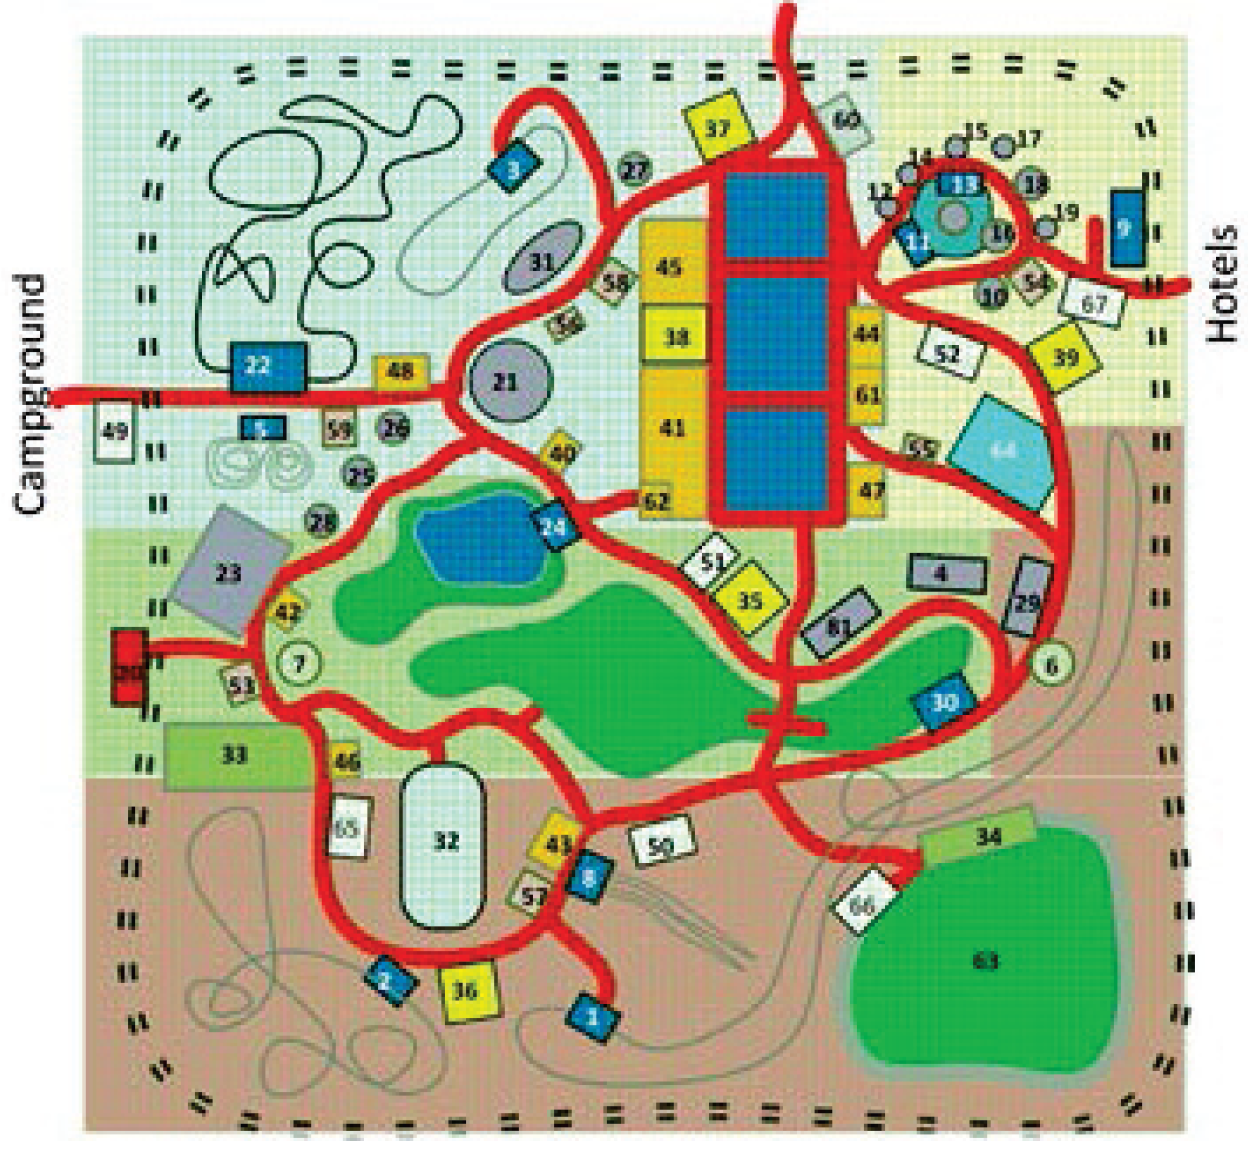
\includegraphics[width=\columnwidth]{img/pic.png}
    \caption{Example image from a VAST challenge.}
      \label{fig:pic}
\end{figure}


\section{Design \& implementation of VA solution}
Design and implementation details. 
What languages, libraries, tools have you used to implement your solution? Why did you choose that?

\section{Discussion}
Discuss aspects relevant to your analysis strategy as well as implemented solution.
Pros/cons of the proposed approach.
Discuss various limitations posed. 
How/what could you have done differently.

\section{Conclusions}
Here you include your concluding remarks. 

You can summarize the overall solution scenario you have come up with. 
Potentially present future work.

\bibliographystyle{abbrv}

%%use following if all content of bibtex file should be shown

\bibliography{refs}

\section*{Contributions from Each Project Member}\label{cont}

\begin{description}
\item[Author x] {Contributions}
\item[Author y] {Contributions}
\item[Author z] {Contributions}

\end{description}


\end{document}
